\section{Question, assumptions and inherited geometry}\label{sec:foundations}
Hilmir Fr\'imann Halld\'orsson's geometric proposal places a transverse local loop through paired upper and lower measurement regions of the folded Tri-Octagon and surrounds the central module with complete smaller copies. His subsequent height and radius comparisons ask whether position changes what those copies can receive. Paper I establishes the geometry and distinguishes it from an observation law.~\cite{PaperI} The present paper supplies a precise conditional source-to-observation construction using the already defined C1 carrier and C6 reception map.~\cite{SRG05,SRG06} The question is what paired inputs generate, and which exterior records distinguish the result.

The development follows the author's sustained human--AI mathematical collaboration. The paired geometry and multi-ring questions motivate the analysis; the particular carrier law, reception kernel and pulse calibrations are stated comparison choices. Mathematical usefulness for computation need not await a physical realization of the carrier. Conversely, a useful formula does not establish computational advantage or a natural mechanism. We keep this distinction at the level of definitions and conclusions, while giving the conditional mathematics in full.

There are three stages of evidence. Geometric and native-readout definitions are inherited from Paper I and its source snapshots. C1 and C6 are explicit adoptions, not deduced from those definitions. The finite pulse and timing controls are prescribed tests of the adopted system; their generated states and identification results are deductions. The numerical matrices reported below are retained SRG-06--08 results, with their original error qualifications.~\cite{SRG07,SRG08,Reviews} No new reception quadrature or trajectory is needed for this consolidation.

\subsection{One circle, actual contacts and complete observers}
Use the width-one folded shell of Paper I, with origin $O=(0,\sqrt3/6,0)$, $u=(0,1,0)$, $v=\ez\times u=(-1,0,0)$ and $\ez=(0,0,1)$. Define
\begin{equation}\label{eq:geometry}
 K=\frac{\sqrt3}{12}+\frac{\sqrt6}{4},\qquad
 a=\frac{K}{1+\sqrt3/2},\qquad R=\frac{\sqrt7a}{2},\qquad L=2\pi R.
\end{equation}
The selected local centreline, with its fixed orientation, is
\begin{equation}\label{eq:circle}
 \Gamma(s)=B_0+R(\cos\chi\,u+\sin\chi\,\ez),\quad
 B_0=O+Ku,\quad \chi=s/R\pmod{2\pi},\quad
 \hat t=-\sin\chi\,u+\cos\chi\,\ez.
\end{equation}
It is a vertical offset circle. The central shell remains the folded annulus; the circle is an additional conditional construction, not a new material edge or a join of the boundary rims. Its two contacts and signed readout normals are
\begin{equation}\label{eq:contacts}
 P_\pm=O+au\pm a\ez,\qquad n_\pm=(2u\pm\sqrt3\ez)/\sqrt7.
\end{equation}
Write $\theta=\arctan(2/\sqrt3)$ and $\eta=R\theta$. The correct quadrants give
\begin{equation}\label{eq:arcs}
 s_+=L/2-\eta,\quad s_-=L/2+\eta,\qquad
 \ell_{\rm short}=2\eta,\quad\ell_{\rm long}=L-2\eta.
\end{equation}
Indeed $\cos\chi_\pm=-\sqrt{3/7}$ and $\sin\chi_\pm=\pm2/\sqrt7$, so the contact tangents are $-n_+$ and $+n_-$. These facts do not insert a sign in the later source law. The arcs are approximately $0.9195560877$ and $2.4510718473$, with $R=0.5364520972$ and $L=3.3706279350$. The contacts are neither antipodal nor snapped to a twelve-site grid.

For observer index $k=0,\ldots,11$, let $\psi_k=\pi/2+k\pi/6$, $e_r=(\cos\psi_k,\sin\psi_k,0)$ and $e_\psi=(-\sin\psi_k,\cos\psi_k,0)$. The inherited centres, frames and full miniature vertices are
\begin{equation}\label{eq:observers}
 X_{mk}=O+\rho_m e_r+h_m\ez,\qquad B_k=[e_r,\ez,-e_\psi],\qquad
 P\longmapsto X_{mk}+\tfrac14 B_k(P-O).
\end{equation}
Every original vertex and face is retained under this map. H uses $\rho_m=3$ and $h_m/a=2,1,0,-1,-2$; R1,R2,R3 use $\rho_m=2,3,4$ at $h_m=0$. The 96 labels describe 84 distinct sites, because H0 and R2 coincide in both centre and frame. A combined height-by-radius product is not instantiated. The quarter-turn fixes the frame; centre sampling below does not turn miniature surface area into a receiving area.

\begin{figure}[htbp]\centering
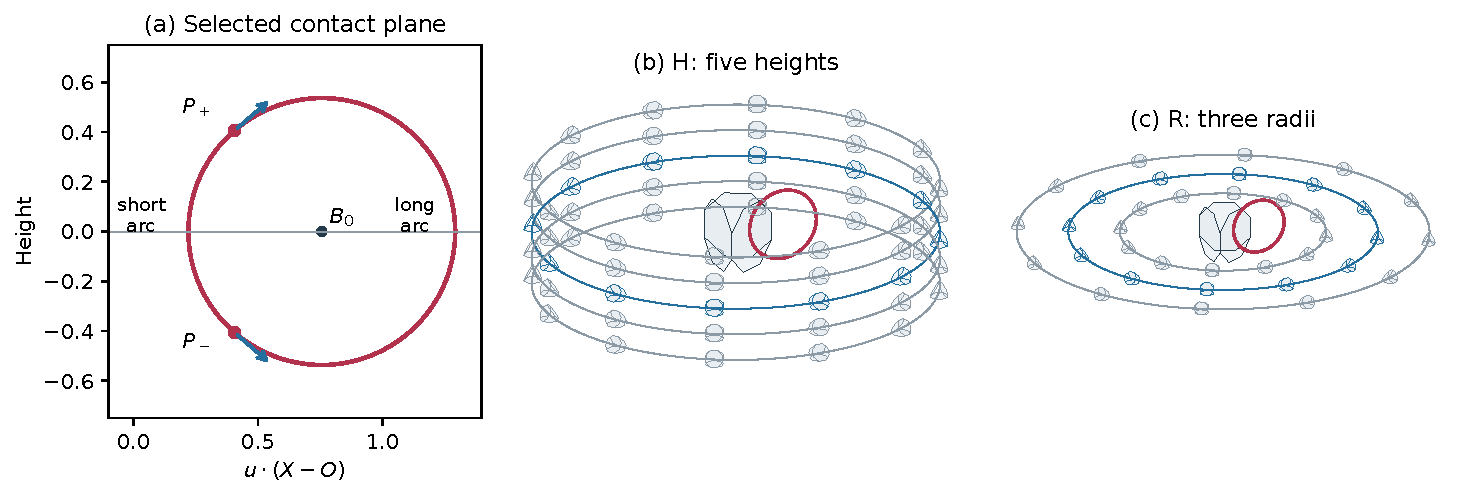
\includegraphics[width=\textwidth]{figures/geometry.pdf}
\caption{Inherited geometry and conditional carrier. The median view shows the actual contacts and unequal arcs of $\Gamma_0$; the paired normals are readout covectors. The separate H/R views retain all complete quarter-scaled modules. Their placement rings are reference curves, not carriers. Blue marks H0/R2, the same twelve sites. No line joining a source to a receiver represents a material connection.}\label{fig:geometry}
\end{figure}

\subsection{Typed input chain and the missing component}\label{sec:typed}
Let $\Omega\in\C^3$ be the native state. The separately defined readouts include
\begin{equation}\label{eq:readouts}
 I=\norm{\Omega}^2,\quad C=\Re\Omega\times\Im\Omega,\quad
 M=z(\cos\vartheta_c,\sin\vartheta_c,1),
\end{equation}
where the staged scalar is
\begin{equation}\label{eq:staged}
 z=\lambda_{vp}\frac{\sqrt I}{1+\sqrt I}
 \cos[3(\vartheta_c-\vartheta_{\rm lock})]e^{-\gamma t_{\rm clock}}.
\end{equation}
The integer clock $q$ supplies $\vartheta_c=2\pi(q\bmod N)/N$. The source also defines the blend $T_{\rm blend}=\alpha M+\beta C$; it is not a third independent state. These formulas are numerical readouts and are not an ambient field law.~\cite{Native}

For one named family $v_{\rm in}=M$ or $C$, fix the inherited dictionary $A=\lambda_gR_z(\delta_g)$. The chain is
\begin{equation}\label{eq:sourcechain}
 \Omega,\text{ clock/configuration}\longmapsto v_{\rm in}
 \longmapsto W=Av_{\rm in}\longmapsto q_\pm=n_\pm\tr W
 \longmapsto f_\pm=\kappa_{\rm in}q_\pm.
\end{equation}
The positive common gain $\kappa_{\rm in}$ is an adopted conversion of data units to source strength. It is not an energy efficiency. Writing $W=W_ru+W_av+W_z\ez$, define
\begin{equation}\label{eq:sectors}
 f_s=\tfrac12(f_++f_-)=\frac{2\kappa_{\rm in}}{\sqrt7}W_r,
 \qquad f_a=\tfrac12(f_+-f_-)=\frac{\sqrt3\kappa_{\rm in}}{\sqrt7}W_z.
\end{equation}
The kernel of this pair projection is exactly $\operatorname{span}(v)$. Equal projected histories and equal carrier preparation give equal downstream states and records by uniqueness. An added observer cannot recover $W_a$ or a native cubic invariant $J$ lost upstream. At fixed readout clock, $M$ has only one real scalar freedom, even though the abstract two-port calibration has two input coefficients.

\subsection{Conventions and dimensions}\label{sec:units}
The width normalization is geometric. Multiplying all coordinates by a length unit restores dimensional lengths; no SI length or time is selected. We denote dimensions by $\mathrm L,\mathrm T,\mathrm U,\mathrm Q$ to avoid confusing them with the circumference $L$ or the pulse duration $T$.
\begin{table}[htbp]\centering\small
\begin{tabular}{P{.29\textwidth}P{.35\textwidth}P{.23\textwidth}}\toprule
Symbol & Meaning & Dimension\\\midrule
$s,R,L,\epsilon,d$ & Arclength, radius, width, distance & $\mathrm L$\\
$t,c,c_e$ & Analysis time; two independent speeds & $\mathrm T$; $\mathrm L/\mathrm T$\\
$p,r$ & Real carrier variables & $\mathrm U$\\
$b_\pm; f_\pm$ & Normalized profiles; source strengths & $\mathrm L^{-1}$; $\mathrm U\mathrm L/\mathrm T$\\
$q_\pm;\kappa_{\rm in}$ & Input data; common conversion & $\mathrm Q$; $\mathrm U\mathrm L/(\mathrm T\mathrm Q)$\\
$e;E$ & Storage density; total storage & $\mathrm U^2$; $\mathrm U^2\mathrm L$\\
$j;f_\pm y_\pm$ & Local oriented flux; source power & $\mathrm U^2\mathrm L/\mathrm T$\\
$\Jflux=\int j\dd s$ & Spatially integrated oriented flux & $\mathrm U^2\mathrm L^2/\mathrm T$\\
$U,V,Y$ & Scalar, vector, local exterior record & $\mathrm U$\\
$g_o$ & Common exterior calibration & Dimensionless\\\bottomrule
\end{tabular}
\caption{Model dimensions. In particular, $\Jflux$ is not power through a section.}\label{tab:units}
\end{table}

Spatial Fourier coefficients use $L^{-1}\int_0^L f(s)e^{-\ii ns/R}\dd s$. Temporal phasors use $e^{+\ii\omega t}$, and finite transforms use $\int f(t)e^{+\ii\omega t}\dd t$. Thus an exterior delay contributes $e^{-\ii\omega d/c_e}$. A directional amplitude subscript denotes propagation, not a source-port label. We use normalized characteristics $w_\sigma=(p+\sigma r)/\sqrt2$ throughout; the unnormalized convention in SRG-08 is $\widetilde w_\sigma=\sqrt2w_\sigma=p+\sigma r$.

The native iteration index, the readout clock $(q,t_{\rm clock})$, carrier time $t$, arclength $s$ and observer index $k$ are independent variables. Later $T=L/c$ is a prescribed pulse scale, not $T_{\rm blend}$. Reception moments are $H,S_m,C_m$; $C_m$ is never the native readout $C$. The frame $B_k$, tent factor $B_n$ and centre $B_0$ have distinct subscripts and types.

\begin{figure}[htbp]\centering
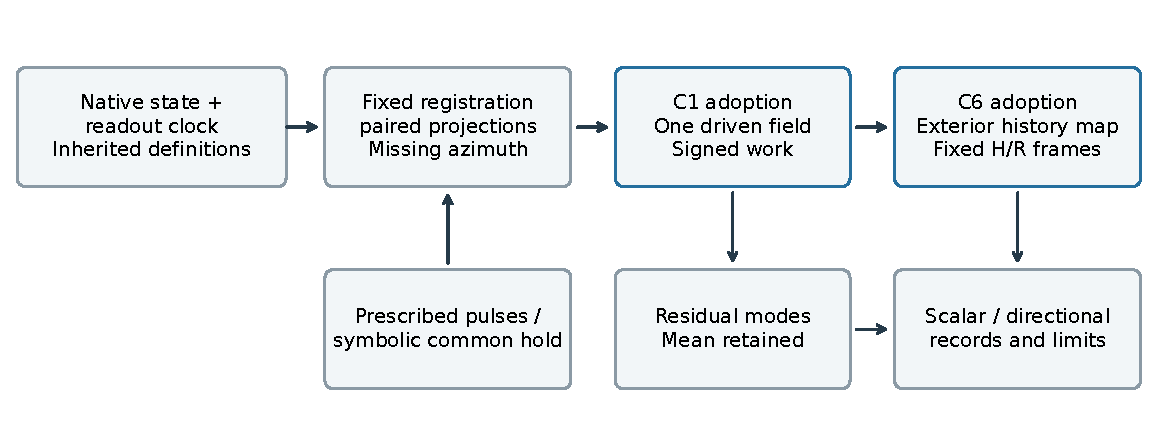
\includegraphics[width=\textwidth]{figures/dependencies.pdf}
\caption{Dependency and information boundaries. Solid boxes are defined objects; arrows state explicit maps. C1 and C6 are separate adoptions. The sample-and-hold bridge in Section~\ref{sec:native} is conditional and uses symbolic cadence. Observer duplication adds records without adding a state or modifying source work.}\label{fig:dependencies}
\end{figure}
